\section{Uppgift 1}\label{uppgift-1}

\subsection{Instruktioner}
\begin{verbatim}
1. I nedanstående program saknas datatyperna (där det står ...) vid
   variabeldeklarationerna. Din uppgift är att fylla i rätt datatyp vid
   respektive deklaration. Provkör sedan programmet:

   public class Datatyper
   {
       public static void main(String[] args)
       {
           ... data1 = true;
           ... data2 = 45.8F;
           ... data3 = 29;
           ... data4 = data3 < 10;
           ... data5 = 12 / 5;
           ... data6 = data3 * data5;
           ... data7 = 10 % 3;
           ... data8 = "Java programmering";
           ... data9 = 'b';
           ... data10 = (float)data5 / 4;

             System.out.println     ("Variabeln     data1: " + data1);
             System.out.println     ("Variabeln     data2: " + data2);
             System.out.println     ("Variabeln     data3: " + data3);
             System.out.println     ("Variabeln     data4: " + data4);
             System.out.println     ("Variabeln     data5: " + data5);
             System.out.println     ("Variabeln     data6: " + data6);
             System.out.println     ("Variabeln     data7: " + data7);
             System.out.println     ("Variabeln     data8: " + data8);
             System.out.println     ("Variabeln     data9: " + data9);
             System.out.println     ("Variabeln     data10: " + data10);
         }
     }
\end{verbatim}

\subsection{Lösning}
\subsubsection{Kommentar}
Det är något oklart vad som efterfrågas. I problembeskrivningen specifieras
inte huruvida målvariabelns datatyp ska vara lämpad för att lagra resultatet av
beräkningen på det vis att ingen data går förlorad genom trunkering eller
avrundning.  Eller om målvariabeln helt enkelt ska ha samma datatyp som de
övriga operanderna. Jag har valt att vara konservativ i fråga om "resurser" 
och använder de datatyper som krävs för att lagra den information som ska
behandlas. Om exekversingstid och/eller lagringsutrymme inte är någon faktor att
beakta kunde alla variabler få vara 64-bitars floats.

%Bla \mintinline{latex}{\mintinline{latex}{your $code$ goes here}} bla.

\par Nämnvärt är att en inmatad siffra utan specifierad datatyp ges typen
integer
%per default. Detta är fallet för \mintinline{java}{data5 = 15 / 5;} : 12 och 5
%har typen int och
per default. Detta är fallet för $data5 = 15 / 5$ ; 12 och 5 har typen int och
resultatet innehåller inga decimaler.  Detaljer rörande 'literals' hämtas bäst
från The Java Language Specification, Java SE 8 Edition
\footnote{\url{https://docs.oracle.com/javase/specs/}}



\subsubsection{Källkod}\label{uppgift-1_src}
%\begin{listing}[]
    \inputminted[linenos]{java}{src/Lab1Uppg01.java}
    \caption{Lab1Uppg01.java}
    \label{Uppg1src}
%\end{listing}

\subsubsection{Skärmdump}
\begin{figure}[htbp]
    \centering
        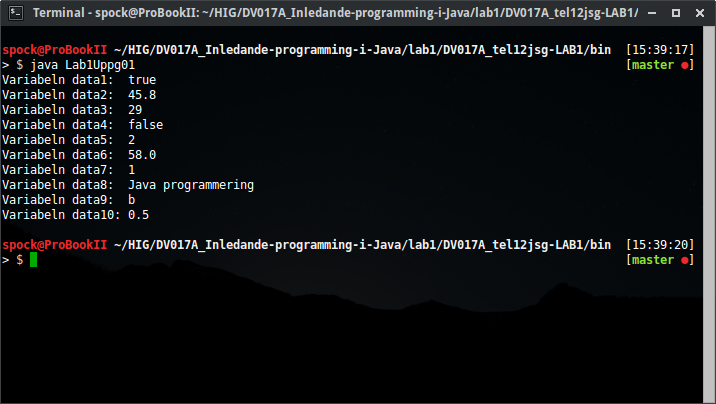
\includegraphics[width=\linewidth]{img/01.png}
    \caption{Körning av koden till Uppgift \ref{uppgift-1}}
    \label{fig:screenshot-01}
\end{figure}

